% !TEX root = ../ACT4E-ready.tex
This chapter introduces basic concepts of engineering design, and describes what are the design queries we want to answer.


\subsection{\readytoreview{What is ``design''?}}

We take a broad view of what it means to ``design'', that is not limited to engineering. Citing at length 
Hebert Simon's\footnote{Hebert A. Simon (1916-2001). Winner of the 1978 Nobel Prize in Economics.}
\emph{The sciences of the artificial}~(\cite{hebert96sciences}, Chapter 5):

\begin{quote}
    Engineers are not the only professional designers. Everyone designs who devises courses of action aimed at changing existing situations into preferred ones. The intellectual activity that produces material artifacts is no different fundamentally from the one that prescribes remedies for a sick patient or the one that devises a new sales plan for a company or a social welfare policy for a state. Design, so construed, is the core of all professional training; it is the principal mark that distinguishes the professions from the sciences. Schools of engineering, as well as schools of architecture, business, education, law, and medicine, are all centrally concerned with the process of design.
\end{quote} 

The metaphors used in the book are biased towards engineering.
It is easy for everybody to imagine to create a physical machine out of simple components,
and what choices and trade-offs we must deal with. Furthermore, it is easy to imagine
what is the boundary between the machine and the world, that is, to delimit the design space.

Yet the theory to be discussed is applicable to other disciplines, if one takes a more
abstract view of what is a system and a component. For example, in urban planning, the
components of a city are roads, sewers, residential areas, etc. In other disciplines,
``components'' can be logical instead of physical. For example, an economist might ask how to
design an incentive scheme such that such scheme (a ``component'') will move the system to a more
desirable set of states.


\subsection{\readytoreview{What is ``co-design''?}}

The word ``co-design'' is not a new one. In this book, we will use 
a meaning that incorporates and extends the existing meaning.

We take the ``Co'' in ``co-design'' to have four meanings:
\begin{enumerate}
    \item ``co'' for ``compositional'';
    \item ``co'' for ``collaborative'';
    \item  ``co'' for ``computational'';
    \item   ``co'' for ``continuous'';
\end{enumerate}
These meanings together describe the aspects of modern engineering design.


\subsubsection{``Co'' for ``compositional''}

The first meaning has to do with composition:

\begin{quote}
     co-design = design everything together
\end{quote}

We use the word ``co-design'' to refer to any decision procedure that has to do with making
simultaneous choices about the components of a system  to achieve system-level
goals. This includes the choice of components, the interconnection of components, and the configuration of components. We will see that in most cases, choices that are made at the level of components without looking at the entire system are doomed to be suboptimal.


Slightly modifying Haiken's quote in~\cref{sec:systems-and-components}, we choose this as our slogan:

\begin{quote}
     A system is composed of components;\\
       a component is something you understand
       \textbf{how to design}.
\end{quote}

\subsubsection{``Co'' for ``collaborative''}

In a second broad meaning, ``co-'' stands for ``collaborative'':

\begin{quote}
    co-design = design everything, together
\end{quote}


There are two types of collaborations. First, there is the collaboration  between human and machine, in the definition and solution of design problems. Second, and most importantly, is the collaboration among different experts or teams of experts in the design process.

The typical situation is that the system design is suboptimal because every expert only knows one component and there are rigid interfaces/contracts designed early on. The problem here is sharing of knowledge across teams, specifically, knowledge about the design of systems.

In this case, this is the slogan:
 
\begin{quote}
    \enquote{A system is composed of components;\\
      a component is something that \textbf{somebody} understands
      \textbf{how to design}.}
\end{quote}


There is a tight link between the ``composition'' and ``collaboration'' aspects.

As Conway\footnote{John Horton Conway (1937--2020) was a mathematician. Probably the most 
popular idea of his was the invention of the Game of Life, which inspired countless
works on cellular automata. We remember him for the discovery of the \emph{surreal numbers},
which should be just called \emph{numbers}, as they contain all other ordered fields.} first observed for software systems:

\begin{quote}
\enquote{Organizations which design systems [...] are constrained to produce designs which are copies of the communication structures of these organizations.}
\end{quote}
 

This ``mirroring'' hypothesis between system and organization was explored formally and found to hold~\cite{maccormack12exploring}. The ultimate reason is that ``the organization's governance structures, problem solving routines and communication patterns constrain the space in which it searches for new solutions''. This appears to be true for generic systems in addition to software.

\todo{use angled quotes for above}

In the end, civilization is about dividing up the work, and so we must choose where one's work ends and the other's work begins. But we need to keep talking if we want that everything works together.
 

\subsubsection{``Co'' for ``computational''}

The third meaning of ``co-'' in ``co-design'' will be \textbf{computational}. It is the age of machines and we need
 machines to understand what we are doing. 

Therefore, we strive to create not only a qualitative modeling for co-design, but also a formal and quantitative description that will be suitable for setting up an optimization problem that can be solved to obtain an optimal design.

Our slogan becomes:

\begin{quote}
    \enquote{A system is composed of components;\\
      a component is something that \textbf{somebody} understands
      \textbf{how to design} \textbf{well enough to teach a computer}.}
\end{quote}


\subsubsection{``Co'' for ``continuous''}

The fourth meaning of ``co-'' is \textbf{continuous}. We look at designs not as something that exists
as a single decision in time, but rather as something that continuous to exist and evolve, independently 
on the designer.


% <!-- Also, in addition to considering design as a creative process,
% typical
% some of the theory to be developed is used in post-hoc analysis.
% In the biological sciences the system is already designed (evolved)
% but the idea of biological organisms as systems is pretty clear. -->

% <!--
% Complexity also depends on what exactly is the task at hand with which we are confronted. Given
% a system, is the problem to simulate it? to decompose it? to predict future states? to assess
% the causes of a failure? -->



\subsection{\statusdraft{Basic concepts of formal engineering design}}

We will informally introduce some of the basic nomenclature of engineering
design~\cite{antonsson2005formal,deweck2011}. Later, all these concepts will find a formal
definition in the language of category theory.

\paragraph{Functionality and functional requirements} You are an engineer in front of an empty whiteboard, ready to start designing the next product.
The first question to ask is: What is the \emph{purpose} of the product to be designed? The purpose of the product is expressed by the \emph{functional requirements}, sometimes called
\emph{functional specifications}, or simply \emph{function}.

Unfortunately, the word ``function'' conflicts with the mathematical concept. Therefore, we
will talk  about \emph{functionality}. Moreover, we will never use the word ``function'', and
instead use \emph{map} to denote the mathematical concept.

\begin{example}
    These are a few examples of functional requirements:
    \begin{itemize}
        \item A car must be able to transport at least $n \geq 4$ passengers.
        \item A battery must store at least $\unit[100]{kJ}$ of energy.
        \item An autonomous vehicle should reach at least $\unit[20]{mph}$ while guaranteeing safety.
    \end{itemize}
\end{example}

\paragraph{Resources and resource constraints}

We call \emph{resources} what we need to pay to realize the given functionality.
In some contexts, these are better called \emph{costs}, or \emph{dependencies}.


\begin{example}
These are a few examples of resource constraints:
\begin{itemize}
\item A car should not cost more than \unit[15,000]{USD}.
\item A battery should not weigh more than \unit[1]{kg}.
\item A process should not take more than \unit[10]{s}.
\end{itemize}
\end{example}

\paragraph{Duality of functionality and resources}

There is an interesting duality between functionality and resources. When designing systems, one is given functional requirements, as a \emph{lower bound} on the functionality to provide, and one is given resource constraints, which are an \emph{upper bound} on the resources to use.

As far as design objectives go, most can be understood as either \emph{minimize resource usage}
or \emph{maximize functionality provided}.

This duality between functionality and resources will be at the
center of our formalization.

\paragraph{Non-functional requirements}

Functionality and resources do not cover all the requirements--- there is, for example, a
large class of \emph{non-functional requirements}~\cite{deweck2011} such as the extensibility and the
maintainability of the system. Nevertheless, functionality and resources can express most of
the requirements which can be quantitatively evaluated, at least prior to designing, assembling,
and testing the entire system.

\paragraph{Implementation space}

The \emph{implementation space} or \textit{design space} is the set of all possible design choices that could be chosen; by \textit{implementation}, or the word ``design'', used as a noun, we mean one particular  set of choices. The implementation space $\impsp$ is the set over which we are optimizing; an implementation $\imp\in\impsp$ is a particular point in that set~(\cref{fig:impspace}).

\begin{figure}[h!]
    \begin{center}
    \includesag{15_imp_space}
    \end{center}
    \caption{An \emph{implementation} $\imp$ is a particular point in the implementation space $\impsp$.}
    \label{fig:impspace}
\end{figure}
\todo{Make cute implementation set as in the definition of DPI}


The interconnection between functionality, resources, and implementation spaces
is as follows. We will assume that, given one implementation, we can evaluate it
to know the functionality and the resources spaces~(\cref{fig:FIR}).

\todo{Make cute diagrams as in the definition of DPI}
\begin{figure}[h!]
    \centering
    \includesag{30_dpcatfig_fir}
    %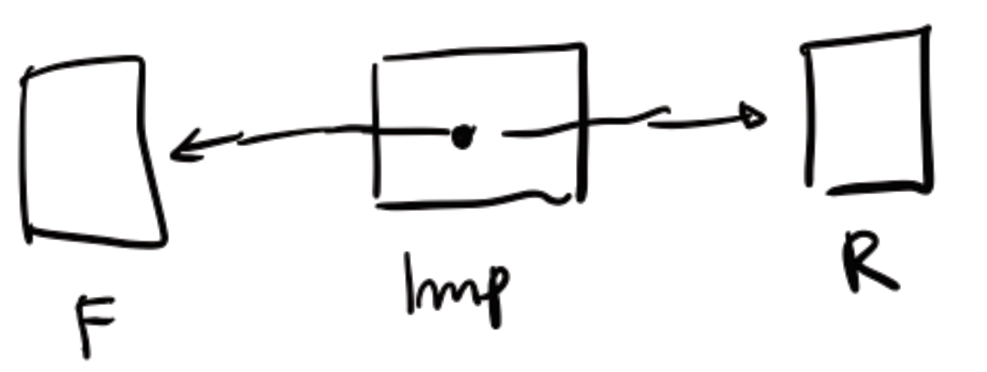
\includegraphics[scale=0.33]{dpcatfig_fir}
    \caption{Evaluation of specific implementations to get functionality and resources spaces.\label{fig:FIR}}
\end{figure}
 


\paragraph{Functional Interfaces and interconnection}

Components are \emph{interconnected} to create a system.
This implies that we have defined the \emph{interfaces} of components, which
have the dual function of delimiting when one component ends and another begins,
and also to describe exactly what is the nature of their interaction.

We will develop  a formalism in which the functionality and resources
are the interfaces used for interconnection: two components are connected
if the resources required by the first correspond to the functionality
provided by the second.


\paragraph{Abstraction}

By \emph{abstraction}, one usually means that it is possible to ``zoom out'',
in the sense that a system of components can be seen as a component itself,
which can be part of larger systems.

\JL{I think here we might want to be careful... people (and in particular mathematicians) maybe mean lots of different things by `abstraction' and here it is being used in a very specific sense... perhaps we don't say `one usually means'... or perhaps there is a different word which fits?}


\paragraph{Compositionality}

A \emph{compositional} property is a property that is preserved by interconnection and abstraction; assuming each component in a system satisfies that property, also the system as a whole satisfies the property.

\begin{example}
One can compose two electronic circuits by joining their terminals to obtain
another electronic circuit. We would say that the property
of being an electronic circuit is compositional.
\end{example}

\JL{Would be nice to also give an example of something that is *not* compositional}


\subsection{Queries in design}
 
Suppose that we have a model with a functionality space~$\funsp$, a requirements space~$\ressp$, and an implementation space~$\impsp$. 

There are several queries we can ask of a model. They all look at the same phenomenon from different angles, so they look similar; however the computational cost of answering each one might be very different.

The first kind of query is one that asks if the design if feasible when fixed all variables 

\begin{problem}[Feasibility problem]
    Given a triplet of implementation $\imp\in\impsp$, functionality~$\fun\in\funsp$, requirements $\res\in\ressp$, determine if the design is feasible. 
\end{problem}


The second type of query is that which fixes the boundary conditions of functionality and requirements, and asks to find a solution.

\begin{problem}[Find implementation]
    Given a pair  of  minimal requested functionality $\fun\in\funsp$ and maximum allowed requirements $\res\in\ressp$, determine if there is a an implementation $\imp\in\impsp$ that is feasible.
\end{problem}

A different type of query is the one in which the design objective (the functionality)
is fixed, and we ask what are the least resources necessary.


\begin{problem}[FixFunMinReq]
    Given a certain functionality $\fun\in\funsp$, find the set of ``minimal'' resources in $\ressp$ that are needed to realize it (along with the implementations), or provide a proof that there are none. 
\end{problem}


Dually, we can ask, fixed the resources available, what are the functionalities that can be required.

\begin{problem}[FixReqMinFun]
    Given a certain requirement $\res\in\ressp$, find the set of ``maximal'' functionalities in that can be realize it (along with the implementations), or provide a proof that there are none. 
\end{problem}


It is very natural to talk about the ``minimal'' requirements and ``maximal'' functionalities;
after all, we always want to minimize costs and maximize performance. In the next chapter
we start to put more mathematical scaffolding in place, starting from definining functionality
and requirements as posets.

% The design queries we will present throughout this paper are the following:
% \begin{item}
% \item 
    
% \item 
% \item Given certain resources, find the maximal functionality that can be realized, or provide a proof that there are none.
% \end{item}



